\chapter{BIODATA PENULIS}
\begin{wrapfigure}{l}{0.4\textwidth}
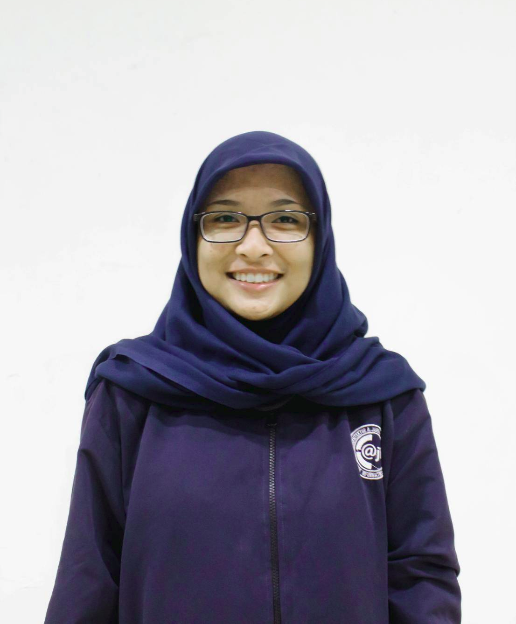
\includegraphics[height=0.3\textheight]{biodata/hana.png}
\end{wrapfigure}

\textbf{Rohana Qudus}, lahir di Gresik tanggal 7 Februari 1998. Penulis merupakan anak kedua dari 2 bersaudara. Penulis telah menempuh pendidikan formal TK Dharmawanita Gresik, SD Muhammadiyah 2 Gresik (2004-2010), SMP Negeri 1 Gresik (2010-2013) dan SMA Negeri 1 Gresik (2013-2015). Penulis melanjutkan studi kuliah program sarjana di Departemen Informatika ITS. 

Selama berkuliah di Departemen Informatika ITS, penulis  pernah menjadi asisten dosen dan praktikum untuk mata kuliah Sistem Operasi (2017) dan Jaringan Komputer(2018). Selama menempuh perkuliahan penulis juga aktif di kegiatan organisasi dan kepanitiaan diantaranya menjadi Staf Departemen Media Informasi HMTC ITS, Staf Departemen Informasi Informasi Media BEM FTIF ITS, Staf Ahli Departemen Media Informasi HMTC ITS, Staf Website dan Kesekretariatan Schematics 2016, dan Staf Ahli 3D Schematics 2017. Penulis dapat dihubungi melalui surel di \\ \texttt{rohanaq27@gmail.com}.

\chapter{BIODATA PENULIS} 
\begin{wrapfigure}{l}{0.4\textwidth} 
	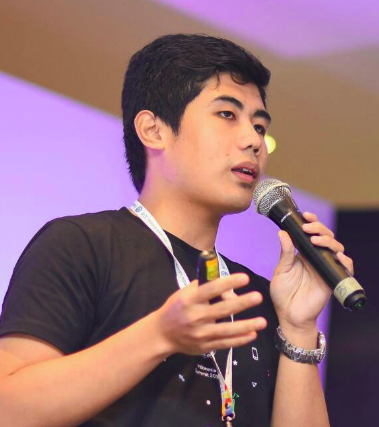
\includegraphics[height=0.3\textheight]{biodata/rafi.png} 
\end{wrapfigure} 

\textbf{Rafi R. Ramadhan}, lahir di Padang Panjang tanggal 27 Januari 1997. Penulis merupakan anak kedua dari 2 bersaudara. Penulis telah menempuh pendidikan formal TK Aisyiyah I Duri, Riau, SD IT Mutiara Duri (2003-2009), SMP IT Mutiara (2009-2012) dan SMA IT Mutiara Duri Riau (2012-2015). Penulis melanjutkan studi kuliah program sarjana di Jurusan Teknik Informatika ITS. 

Selama berkuliah di Departemen Informatika ITS, penulis aktif dalam kegiatan kemahasiswaan seperti Himpunan. Penulis merupakan staf pada Departemen Media dan Informasi HMTC 2016-2017, kemudian melanjutkan menjadi staf ahli pada departemen yang sama untuk periode 2017-2018. Selain di himpunan, penulis juga aktif pada Schematics selama 2 tahun berturut-turut. Penulis juga merupakan Volunteer dari International Office ITS. Penulis berada pada divisi Internationalization and Development Division, divisi ini mengemban tugas untuk mencerdaskan dan membantu proses internasionalisasi yang ada di kampus ITS. Penulis juga merupakan Leader dari Developer Student Clubs yang merupakan program gagasan dari Google Developer. penulis merupakan 1 dari 20 orang yang dipilih menjadi Leader untuk DSC se-Indonesia. Penulis dapat dihubungi melalui surel di \\ \texttt{rafi.ramadhan27@gmail.com}.